\documentclass[12pt, letterpaper]{article}

\usepackage[english]{babel} % Sets the language and regional settings for English documents
\usepackage[utf8]{inputenc} % Allows the use of UTF-8 characters in the document
\usepackage[T1]{fontenc} % Specifies t\subsubsection*{Forma canónica reducida}
\usepackage[margin=2cm]{geometry} % Sets the page margins
\usepackage{makeidx} % Enables the creation of indexes
% \usepackage{natbib} % Provides flexible bibliography support
\usepackage{url} % Allows the use of URLs
\usepackage{enumitem} % Customizes the appearance of lists
\usepackage{listings} % Provides syntax highlighting for code listings
\usepackage[dvipsnames]{xcolor} % Allows the use of colors
\usepackage{parskip} % Modifies paragraph spacing
\usepackage{graphicx} % Enables the inclusion of graphics
\usepackage{tikz} % Allows the creation of graphics and diagrams
\usepackage{float}
\usepackage{hyperref} % Enables the creation of hyperlinks
\usepackage{amsmath} % Provides additional math environments and commands
\usepackage{circuitikz} % Allows the creation of electrical circuits
\usepackage{adjustbox} % Adjusts the size of the circuit diagrams
\usepackage{tcolorbox}
\usepackage{diagbox} % Allows the use of diagonal boxes in table cells
\usepackage{colortbl} % Allows coloring of table cells
\hypersetup{
    colorlinks=true,
    linkcolor=blue,
    urlcolor=blue
}
\usepackage{breakurl} % permite que los links se rompan en varias líneas
\definecolor{mygray}{gray}{0.9}

\usetikzlibrary{shapes.geometric, positioning}

\lstset{
	language=SQL,
	basicstyle=\ttfamily\small,
	keywordstyle=\color{blue},
	commentstyle=\color[rgb]{0,0.5,0},
	stringstyle=\color{red},
	numbers=left,
	numberstyle=\tiny\color{gray},
	stepnumber=1,
	numbersep=10pt,
	backgroundcolor=\color{white},
	showspaces=false,
	showstringspaces=false,
	breaklines=true,
	frame=single,
	tabsize=2, captionpos=b, lineskip=-1pt,
	extendedchars=true,
	literate={á}{{\'a}}1 {é}{{\'e}}1 {í}{{\'i}}1 {ó}{{\'o}}1 {ú}{{\'u}}1 {Á}{{\'A}}1 {É}{{\'E}}1 {Í}{{\'I}}1 {Ó}{{\'O}}1 {Ú}{{\'U}}1 {ñ}{{\~n}}1 {Ñ}{{\~N}}1 {¿}{{\textquestiondown}}1 {¡}{{\textexclamdown}}1
}

% VHDL language configuration
\lstdefinelanguage{VHDL}{
	morekeywords={entity, architecture, signal, port, in, out, inout, begin, end, process, if, then, else, elsif, case, when, others, for, while, loop, wait, library, use, std_logic, std_logic_vector, integer, boolean, rising_edge, falling_edge, component, generic, map, downto, to, and, or, not, xor, nand, nor, xnor},
	morecomment=[l]{--},
	morestring=[b]",
	sensitive=false,
	alsoletter={_}
}

% VHDL listings style
\lstdefinestyle{vhdl}{
	language=VHDL,
	basicstyle=\ttfamily\small,
	keywordstyle=\color{blue}\bfseries,
	commentstyle=\color[rgb]{0,0.6,0}\itshape,
	stringstyle=\color{red},
	numbers=left,
	numberstyle=\tiny\color{gray},
	stepnumber=1,
	numbersep=10pt,
	backgroundcolor=\color{white},
	showspaces=false,
	showstringspaces=false,
	breaklines=true,
	frame=single,
	tabsize=2,
	captionpos=b,
	lineskip=-1pt,
	extendedchars=true
}

\graphicspath{ {./img/} } % Sets the path for the graphics

\newlist{biblio}{enumerate}{1}
\setlist[biblio,1]{label=[\arabic*]}

\makeindex

\begin{document}

\begin{titlepage}

	\begin{tikzpicture}[remember picture,overlay]
		\node[anchor=north west, inner sep=30] at (current page.north west) {
			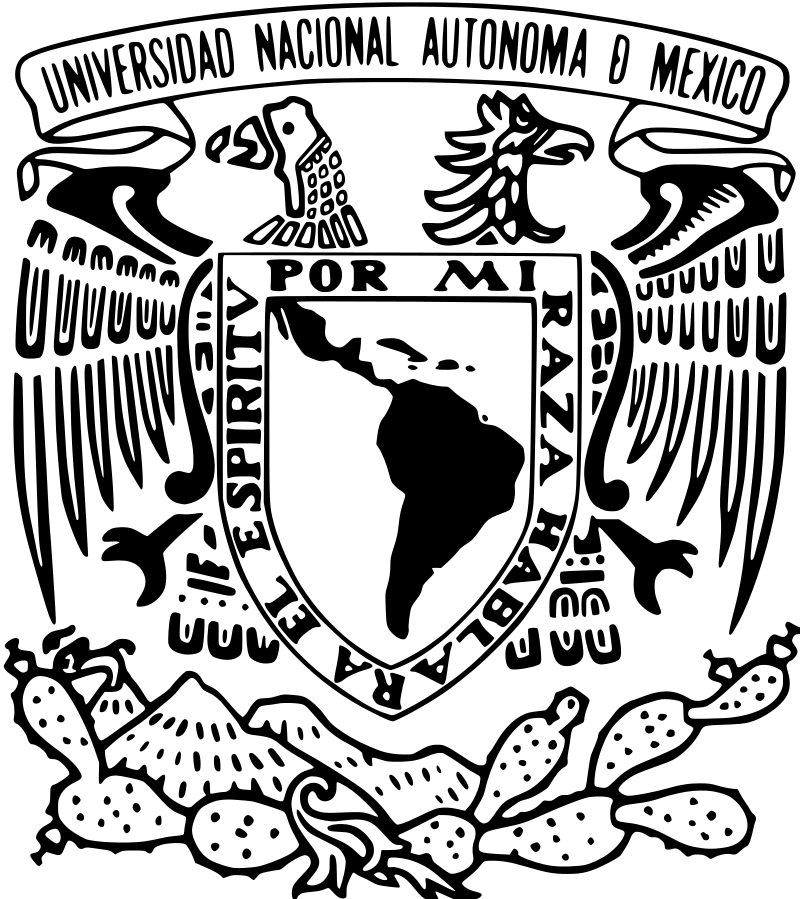
\includegraphics[width=4cm]{escudoUNAM.png}
		};

		\node[anchor=north east, inner sep=30] at (current page.north east) {
			
\includegraphics[width=4cm]{escudoFI.png}
		};
	\end{tikzpicture}

	\begin{center}
		\vspace*{3cm}

		\Huge
		\textbf{Práctica 3 - Corrección de Factor de Potencia}\\

		\vspace{2.5cm}

		\Huge
		\textbf{Facultad de Ingeniería}\\
		Circuitos Electrónicos\\
		\textbf{Ing. Martha Isela Torres Hernández} \\
		2026-1\\

		\vspace{2.5cm}

		\textbf{Grupo:} 4\\

		\vspace{2.5cm}

		\Huge
		\textbf{Integrantes Brigada 6:}\\
		Ugartechea González Luis Antonio\\
		Tepal Briseño Hansel Yael\\
		\textbf{Fecha de entrega:} 21 de Noviembre del 2025\\
		\vspace{2.5cm}
	\end{center}
\end{titlepage}

\section{objetivos}

\begin{itemize}
	\item Presentación de los teoremas de escalamiento de impedancia y de frecuencia.
	\item Familiarizar al alumno con la aplicación práctica de dichos teoremas.
	\item Apreciar la importancia de tales teoremas en el diseño de filtros eléctricos.
\end{itemize}

\section{Objetivos}

Analizar y aplicar técnicas de corrección del factor de potencia en circuitos de corriente
alterna, comprendiendo el efecto de cargas resistivas, inductivas y capacitivas, así como
la importancia de la potencia activa, reactiva y aparente.

\section{Introducción}

El factor de potencia es una medida de la eficiencia con la que un sistema de corriente alterna utiliza la energía eléctrica. Se define como la relación entre la potencia activa (P), que realiza trabajo útil, y la potencia aparente (S), compuesta por la potencia activa y la potencia reactiva (Q). Un bajo factor de potencia está asociado a un mayor desfase entre el voltaje y la corriente, lo que provoca corrientes más elevadas, pérdidas adicionales y un uso ineficiente del sistema eléctrico.
La corrección del factor de potencia se logra mediante la incorporación de capacitores o inductores que compensan la potencia reactiva presente en la carga. Esto reduce el desfase, mejora la operación del sistema y contribuye a una mayor estabilidad y aprovechamiento de la energía.

\section{Desarrollo}

\subsection{Experimento 1}

\begin{figure}[H]
	\centering
	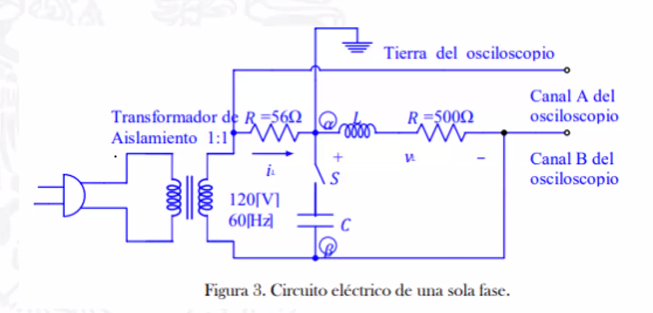
\includegraphics[width=0.8\textwidth]{circuito1.png}
	\caption{Circuito 1}
	\label{fig:circuito}
\end{figure}

Mida el ángulo de desfase entre el voltaje \(V_L\) y la corriente eléctrica \(I_L\). A partir de las mediciones realizadas, determine:

\begin{enumerate}
	\item El factor de potencia de la carga eléctrica.
	\item El triangulo de potencia.
	\item El valor de la capacitancia que se requiere para modificar el factor de potencia a la unidad.
\end{enumerate}

\subsubsection{Datos medidos}
\begin{itemize}
	\item Voltaje de entrada: $V_{rms} = 120V$
	\item Frecuencia: $f = 60Hz$
	\item Corriente: $I_{rms} = 0.186A$
	\item Angulo de desfase: $\phi = 24.1^\circ$
	\item Potencia activa: $P = 0.021 kW$
	\item Potencia reactiva: $Q = 0.009 kVAR$
\end{itemize}

\subsubsection{Cálculos}

Para determinar el factor de potencia (FP) de la carga eléctrica, utilizamos la fórmula:
\[ FP = \cos(\phi) \]
Donde \(\phi\) es el ángulo de desfase medido.
Sustituyendo el valor medido:
\[ FP = \cos(24.1^\circ) \approx 0.913 \]

Por lo tanto, el factor de potencia de la carga eléctrica es:

\begin{tcolorbox}[colback=mygray, colframe=LimeGreen, boxrule=0.7pt, arc=2pt, boxsep=1pt, left=2pt, right=2pt, top=2pt, bottom=2pt, title=Ángulo de desfase]
\begin{equation*}
	\boxed{FP = 0.913}
\end{equation*}
\end{tcolorbox}

Para determinar el triángulo de potencia necesitamos calcular la potencia aparente (S) utilizando la fórmula:
\[S = \sqrt{P^2 + Q^2}\]
Sustituyendo los valores medidos:
\[S = \sqrt{(0.021 kW)^2 + (0.009 kVAR)^2} = 0.0228 kVA\]

Por lo tanto, el triángulo de potencia es:
\begin{center}
	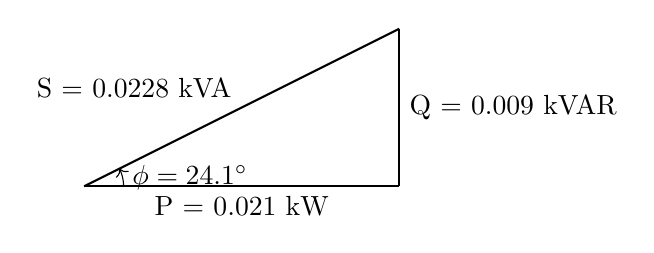
\begin{tikzpicture}
		\draw[thick] (0,0) -- (4,0) node[midway, below] {P = 0.021 kW};
		\draw[thick] (4,0) -- (4,2) node[midway, right] {Q = 0.009 kVAR};
		\draw[thick] (0,0) -- (4,2) node[midway, above left] {S = 0.0228 kVA};
		\draw[->] (0.5,0) arc[start angle=0,end angle=26.57,radius=0.5] node[midway,right] {$\phi = 24.1^\circ$};
	\end{tikzpicture}
\end{center}

Para calcular el valor de la capacitancia necesaria para corregir el factor de potencia a la unidad, utilizamos la fórmula:
\[ C = \frac{Q_C}{2\pi f V^2} \]

Pero para obtener \(Q_C\), es necesario más datos acerca del nuevo angulo que se desea obtener o el factor de potencia deseado. Por fortuna conocemos el angulo de desfasmiento que tendremos al colocalr el capacitor, que es de \(9.5^\circ\). Por lo tanto, podemos calcular \(Q_C\) como:
\[ Q_C = Q_1 - P \tan(\phi_{9.5^\circ}) \]

Sustituyendo los valores:
\[ Q_C = 0.009 kVAR - 0.021 kW \tan(9.5^\circ) \]
\[ Q_C = 0.006 kVAR \]

Ahora podemos calcular la capacitancia:
\[ C = \frac{0.006 kVAR}{2\pi (60 Hz) (120 V)^2} \]

\begin{tcolorbox}[colback=mygray, colframe=LimeGreen, boxrule=0.7pt, arc=2pt, boxsep=1pt, left=2pt, right=2pt, top=2pt, bottom=2pt, title=Ángulo de desfase]
\begin{equation*}
	\boxed{C \approx 1.1 \mu F}
\end{equation*}
\end{tcolorbox}

A continuación, conecte un capacitor cuyo valor de capacitancia sea el más prócximo al calculado, entre los nodos a y B. Observe el efecto en el osciloscopio.

\begin{enumerate}
	\item ¿Qué sucede? Explique. Repita lo anterior para diferentes valores de la capacitancia y conteste las siguientes preguntas.
	\item ¿Qué ocurre cuando el valor de la capacitancia es menor que el calculado?
	\item ¿Y cuando es mayor?
\end{enumerate}

\begin{figure}[H]
	\centering
	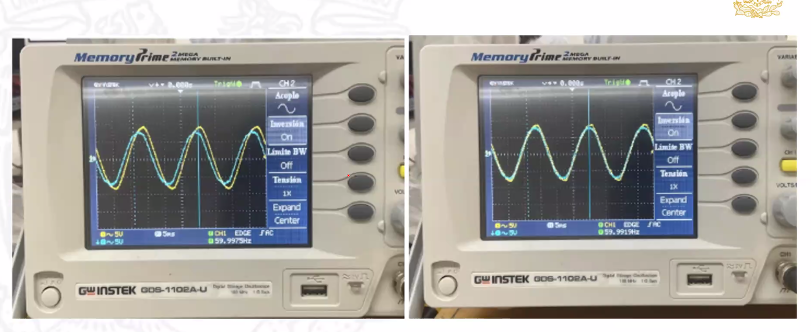
\includegraphics[width=0.8\textwidth]{osciloscopio.png}
	\caption{Osciloscopio con capacitor conectado y sin capacitor}
	\label{fig:circuito}
\end{figure}

Para la primera pregunta, al conectar un capacitor cercano al valor calculado, se observa una reducción en el ángulo de desfase entre el voltaje y la corriente, lo que indica una mejora en el factor de potencia. Esto se debe a que el capacitor proporciona potencia reactiva capacitiva que compensa la potencia reactiva inductiva de la carga, acercando el factor de potencia a la unidad.

Para la segunda pregunta, cuando el valor de la capacitancia es menor que el calculado, el ángulo de desfase de igual forma disminuye debido a que la potencia reactiva de este capacitor sigue compensando la parte inductiva de la carga.

Para la tercera pregunta, cuando el valor de la capacitancia es mayor que el calculado, se observa un cambio en el ángulo de desfase, pero en este caso, el ángulo puede volverse negativo, indicando que la carga ahora tiene un comportamiento capacitivo predominante. Esto puede llevar a un sobrecompensación, donde la potencia reactiva capacitiva excede la potencia reactiva inductiva, lo que también afecta negativamente al factor de potencia.

\subsection{Experimento 2}

\begin{figure}[H]
	\centering
	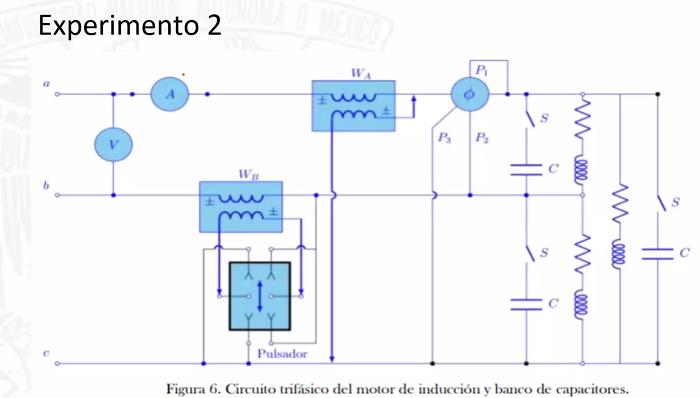
\includegraphics[width=0.8\textwidth]{exp_2.png}
	\caption{Circuito 2}
	\label{fig:circuito}
\end{figure}

Mida el ángulo de desfase. Con este valor y la ecuacion (12), se puede calcular la potencia total suminstrada por los capasitores.

\[Q_{3\phi} = P_{e\phi} (\tan (\phi_1) - \tan (\phi_2))\]

Donde \(\phi\) es el ángulo de desfase original y \(\phi_2\) es el ángulo nuevo de desfase.

\begin{enumerate}
	\item ¿Cual es la potencia reactiva sumisntrada por los capacitores en cada fase?
	\item Determine el valor de la capacitancia que se requiere para suministrar la potencia reactiva que se calculó en la pregunta anterior. ¿Qué concluye?
\end{enumerate}

\begin{table}[H]
\centering
\caption{Tabla de resultados}
\label{tab:tabla8x3}
\begin{tabular}{|c|c|c|}
\hline
 & Sin capacitor 2 & Con Capacitor 3 \\
\hline
Voltaje [V] & 217.9 & 217.9 \\
\hline
Corriente [A] & 2.444 & 0.498 \\
\hline
Potencia activa [W] & 0.796 & 0.164 \\
\hline
Potencia aparente [VA] & 0.919 & 0.181 \\
\hline
Potencia Reactiva [VAR] & 0.476 & 0.061 \\
\hline
F.P & 0.858 & 0.902 \\
\hline
Ángulo de desfase [°] & 31 & 23.8 \\
\hline
\end{tabular}
\end{table}

\subsubsection{Cálculos}

Segun las datos medidos, tenemos que la potencia reactiva para cada fase es:

\begin{tcolorbox}[colback=mygray, colframe=LimeGreen, boxrule=0.7pt, arc=2pt, boxsep=1pt, left=2pt, right=2pt, top=2pt, bottom=2pt, title=Ángulo de desfase]
\begin{equation*}
	\phi_1; Q = 0.476 kVAR
\end{equation*}
\begin{equation}
	\phi_2; Q = 0.061 kVAR
\end{equation}
\end{tcolorbox}

Para determinar el valor de la capacitancia que se requiere para suministrar la potencia reactiva calculada, utilizamos la fórmula:
\[ C = \frac{Q_C}{2\pi f V^2} \]

Calculando \(Q_c\) despejamos la ecuacion proporcionada obteniendo:

\[ Q_C = P_{1} \tan (\phi_1) - P_{2} \tan (\phi_2) \]

Sustituyendo los valores:

\[ Q_C = 0.796 kW \tan (31^\circ) - 0.164 kW \tan (23.8^\circ) \]

\[ Q_C = 0.406 kVAR \]

Ahora podemos calcular la capacitancia:

\[ C = \frac{0.406 kVAR}{2\pi (60 Hz) (217.9 V)^2} \]

\begin{tcolorbox}[colback=mygray, colframe=LimeGreen, boxrule=0.7pt, arc=2pt, boxsep=1pt, left=2pt, right=2pt, top=2pt, bottom=2pt, title=Ángulo de desfase]
\begin{equation*}
	\boxed{C \approx 22.68 \mu F}
\end{equation*}
\end{tcolorbox}

\begin{figure}[H]
	\centering
	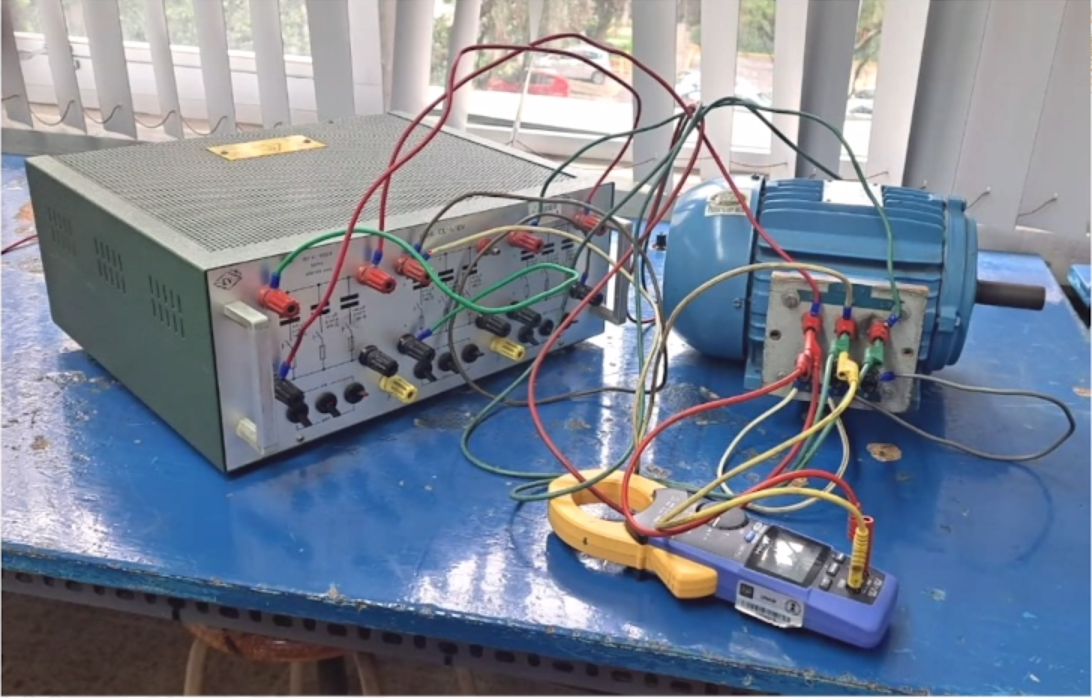
\includegraphics[width=0.8\textwidth]{evidencias.png}
	\caption{Circuito trifasico}
	\label{fig:circuito}
\end{figure}

\section{Conclusiones}

\subsection*{Hansel Yael Tepal Briseño}

A través de los ejercicios realizados, pude observar de forma concreta cómo las mediciones experimentales y los cálculos teóricos se relacionan directamente en la corrección del factor de potencia. Al analizar los valores reales de voltaje, corriente y ángulo de desfase, comprendí cómo se construye el triángulo de potencias y cómo cada componente —activa, reactiva y aparente— influye en el desempeño del circuito. La determinación del capacitor adecuado permitió identificar la diferencia entre una compensación insuficiente y una sobrecompensación, evidenciando que la selección correcta de la capacitancia no solo modifica el ángulo de desfase sino que transforma por completo el comportamiento del sistema.

En el caso trifásico, la comparación entre el circuito con y sin capacitores mostró de forma clara cómo disminuye la potencia reactiva y mejora el factor de potencia en cada fase, lo que refuerza la importancia del análisis fase por fase en instalaciones reales. En conjunto, la práctica me permitió entender que la corrección del factor de potencia no es únicamente un procedimiento matemático, sino una herramienta fundamental para optimizar la operación de sistemas eléctricos tanto monofásicos como trifásicos.

\subsection*{Luis Antonio Ugartechea González}

A lo largo de esta práctica quedó claro que corregir el factor de potencia es esencial para incrementar la eficiencia de los sistemas eléctricos. En el primer ejercicio, correspondiente al circuito monofásico, pudimos analizar cómo la incorporación de un capacitor modificó el comportamiento del circuito, evidenciando una disminución en el consumo de energía innecesaria. En el segundo ejercicio, aplicado a un sistema trifásico, se emplearon nuevamente capacitores para compensar la potencia reactiva, observándose una mejora aún más notable en el funcionamiento del sistema.

En conjunto, la corrección del factor de potencia resulta fundamental, ya que reduce el desperdicio energético, disminuye las pérdidas en las líneas, evita posibles penalizaciones por bajo rendimiento y contribuye a una mayor estabilidad y eficiencia económica de las instalaciones eléctricas.
% \renewcommand{\refname}{}
% \begin{thebibliography}{9}
%    \bibitem{} Dr. E. García, \textit{"Diseño Digital VLSI Repaso DDM"}, presentado en el curso de Diseño Digital VLSI, Ciudad de México, 2025.
% \end{thebibliography}

\end{document}
